\ifdefined\COMPLETE
\else
    \input{./preambule-sacha-utf8.ltx}
    \begin{document}
\fi


\vspace*{-2cm}

\setcounter{section}{0} 

\part{Probabilités}

\vspace*{-.2cm}

\section{Généralités}

\vspace*{-.1cm}

\subsection{Ensembles finis}

\vspace*{-.1cm}

\subsubsection{Définitions}

\begin{itemize}
\item[*] Soit $E$ un ensemble. \\ $E$ est \hbox{un ensemble fini si et seulement si $E$ est vide, ou si E est constitué d'un nombre défini d'éléments.}
\item[*] Soit E un ensemble fini non vide. On appelle \underline{cardinal de E} et on note $\mathrm{Card} \; E$ le nombre d'éléments de E.
\end{itemize} 

\vspace*{.3cm}

\textbf{Exemple}

\vspace*{-1cm}

\centerline{\begin{tabular}{c@{$\qquad \qquad$}c}
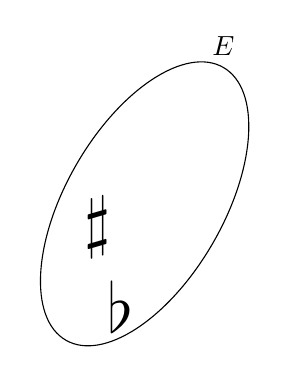
\begin{tikzpicture}
% \draw [help lines] (-2,-2) grid (2,2)  ;
% \tkzTabInit[help]
{\begin{scope} [rotate=-30]
\draw (0,0)  circle  (1 and 2); 
% \draw (0,0) ++(0:-.2) circle (.6 and 1); 
\end{scope} 
\draw (1,2) node {$E$} ; 
\draw (.2,.9) node {\Large $\bigstar$} ; 
\draw (.3,-.1) node { \Large $\blacksquare$} ; 
\draw (-.6,-.3) node { \Huge $\sharp$} ; 
\draw (-.3,-1.3) node {\Huge $\flat$} ; 
}
\end{tikzpicture} 
                     &    \raisebox{8ex}{Card E = 4} \\
                     & \\
\end{tabular}} 

On complète la définition en posant : $\mathrm{Card} \; \varnothing = 0 $.

\vspace*{-.1cm}

\subsubsection{Propriétés}

Soient E et F deux ensembles finis.

\textbf{a)} 


\centerline{
\begin{tabular}{c@{$\qquad \qquad$}c}
                       & \\
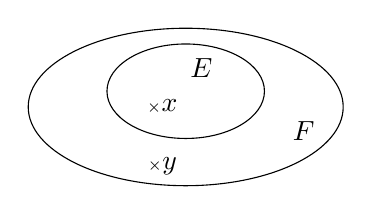
\begin{tikzpicture}
% \draw [help lines] (-2,-2) grid (2,2)  ;
\begin{scope}   [rotate=-90]
\draw (0,0)  circle  (1 and 2); 
\draw (0,0) ++(0:-.2) circle (.6 and 1); 
\end{scope} 
\draw (1.5,-0.3) node {$F$} ; 
\draw (.2,.5) node {$E$} ; 
\draw (-.3,0) node {{\tiny $\times$} $\!\!x$} ; 
\draw (-.3,-.75) node {{\tiny $\times$} $\!\!y$} ; 
\end{tikzpicture}
                     &    \raisebox{5ex}{\parbox{5cm}{
                               \begin{itemize}
                                  \item[*] $\forall x\in E$, $x\in F$.
                                  \item[*] $\exists y\in F$ tel que $y\notin E$                               
                               \end{itemize} 
                               \bigskip                            
                               Si $E\subset F$, alors Card $E \leq$ Card $F$.
                               }} \\
                      & \\         
\end{tabular}} 


\textbf{b)} 

\vspace*{-.5cm}

\begin{center}

\begin{tabular}{c@{$ \;$}c}
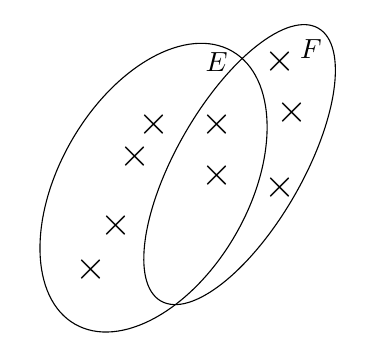
\begin{tikzpicture}[scale=.8]
% \draw [help lines] (-2,-2) grid (3,3)  ;

\begin{scope} [rotate=-30]
    \draw (0,0) circle (1.5 and 2.5); 
    \draw (1,1) circle (1   and 2.5); 
\end{scope} 

\draw (1,2) node {$E$} ; 
\draw (2.5,2.2) node {$F$} ; 

\draw (-1,.-1.3)  node {\Large $\times$} ; 
\draw (-.6,-.6)   node {\Large $\times$} ; 
\draw (-.3,.5)    node {\Large $\times$} ; 
\draw (1,.2) node {\Large $\times$} ; 
\draw (1,1)   node {\Large $\times$} ; 
\draw (0,1)   node {\Large $\times$} ; 
% \draw (.8,1)   node {\Large $\times$} ; 
\draw (2,0)   node {\Large $\times$} ; 
\draw (2.2,1.2)   node {\Large $\times$} ; 
\draw (2,2) node {\Large $\times$} ; 
\end{tikzpicture} 
                     &    \raisebox{15ex}{\parbox{7cm}{
                               On a : $\mathrm{Card} \; E = 6 \qquad $ et $\qquad \mathrm{Card} \; F = 5$.\\
                           

                              Card $\left(E \cup F\right) = 9$. \\
                             
                             
                             $\mathrm{Card} \; \left(E \cap F\right) = 2$.\\ 
                             
                             Plus généralement, on a :  \\ $\mathrm{Card} \; \left(E \cup F\right) 
                 = \mathrm{Card} \; E +\mathrm{Card} \; F - \mathrm{Card} \; \left(E\cap F\right)$.    
                          }} \\
                          
\begin{minipage}{9cm}
\textbf{Remarque : Cas particulier} \\

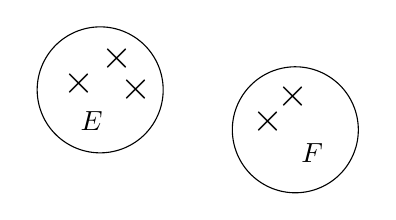
\begin{tikzpicture}[scale=.8]
% \draw [help lines] (-2,-2) grid (3,3)  ;

\begin{scope} [rotate=-30]
    \draw (-1,0) circle (1 and 1); 
    \draw (2,1) circle (1 and 1); 
\end{scope} 

\draw (-1,0) node {$E$} ; 
\draw (2.5,-.5) node {$F$} ; 

\draw (-1.2,.6)  node {\Large $\times$} ; 
\draw (-.6,1)   node {\Large $\times$} ; 
\draw (-.3,.5)    node {\Large $\times$} ; 
\draw (1.8,0) node {\Large $\times$} ; 
\draw (2.2,.4)   node {\Large $\times$} ; 
\end{tikzpicture} 
\end{minipage}
&
\begin{minipage}{8cm}
Si $E \cap F = \varnothing$, alors $\mathrm{card}\left(E\cup F\right) = \mathrm{card}\; E + \mathrm{card} \; F$.
\end{minipage}
\end{tabular} 
\end{center}

\vspace*{-10cm}

\newpage 

\vspace*{-1cm}

\textbf{c)} On a : $E = \lb A ; B ; C\rb $ et $F = \lb 1 ; 2\rb $. Donc $\mathrm{Card} \; E = 3$ et $\mathrm{Card} \; F = 2$. \\

Ainsi, $E {\Large\times} F = \lb \left(a;1\right)\left(a;2\right)\left(b;1\right)\left(b;2\right)\left(c;1\right)\left(c;2\right) \rb $, et $\mathrm{Card} \; \left(E {\Large\times} F\right) = 6$. \\

Donc, $\mathrm{Card} \; \left(E {\Large\times} F\right) = \left(\mathrm{Card} \; E\right)\left(\mathrm{Card} \; F\right)$. \\

$E \times F$ est l’ensemble des couples que l’on peut former avec les éléments des ensembles E et F.
Le signe « $\times$ » est une opération de produit cartésien (ce n’est donc pas une multiplication « habituelle » ).

\subsection{Vocabulaire des probabilités}

\begin{tabular}{c|c|c}
Vocabulaire ensembliste & Vocabulaire statistique & Vocabulaire probabiliste \\
\hline
Ensemble $E$ & Population & Univers $\Omega$. \\
\hline
Élément $x$, avec $x\in E$ & Individu & Éventualité ou cas possible. \\
& & Un univers est constitué d'éventualités. \\
\hline
Sous-ensemble A, avec $A\subset E$ & Échantillon & Événement $A \subset \Omega$. \\
\hline
Partie vide & \Large{$\times$} & Événement impossible \\
\hline
Partie pleine & \Large{$\times$} & Événement certain \\
\hline
Singleton & \Large{$\times$} & Événement élémentaire \\
\end{tabular}

\vspace*{.8cm}

\centerline{
Soit $\Omega$ un univers.}

\centerline{Soient A et B deux événements de $\Omega$.
}

\vspace*{-1.2cm}

\begin{tabular}{ll}
\begin{minipage}{8cm}
\textbf{1.} $\overline{A}$ est l'événement contraire de A. \\ $x \in \overline{A} \Longleftrightarrow x \notin A $. \\


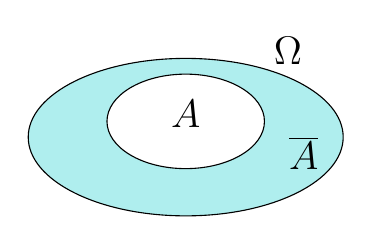
\begin{tikzpicture}
    \begin{scope}   [rotate=-90]
%     \draw [pattern color=blue, pattern=north east lines]  (0,0)  circle  (1 and 2);
    \fill [color=PaleTurquoise]  (0,0)  circle  (1 and 2);    
    \fill [color=white]  (0,0) ++(0:-.2) circle (.6 and 1);
    \draw (0,0)  circle  (1 and 2); 
    \draw (0,0) ++(0:-.2) circle (.6 and 1); 
    \end{scope} 
    \draw (1.5,-0.2) node {\Large $\overline{A}$ } ; 
    \draw (0,.3) node {\Large $A$} ; 
    \draw (1.3,1.1) node {\Large $\Omega$} ; 
    \end{tikzpicture} \\
\end{minipage}
&
\begin{minipage}{8cm}
\vspace*{2cm}
\textbf{2.} $ A \cap B $ est l'événement intersection de A et de B. \\ $x\in A\cap B \Longleftrightarrow x \in A \;  \mathbf{et} \; x \in B $.  \\ 

\def\A_rond{(0,0)  circle  (1 and 2)}
\def\B_rond{(1,1)  circle  (1 and 2)}
\def\GrandRond{(2:0) circle (2.5 and 4)}

% On trace les ensembles 
\begin{tikzpicture}[scale=.6]

% On materialise l'intersection      
    \begin{scope}  [rotate=-30]
      \clip \A_rond;
      \clip \B_rond;
      \fill[color=PaleTurquoise] \GrandRond;
    \end{scope}
% On trace les bords ensuite       
    \begin{scope}  [rotate=-30]
    \draw \A_rond node[left] {$A$};
    \draw \B_rond node [right] {$B$};
    \draw \GrandRond node [above=2] {$\Omega$};
     \end{scope}     
\end{tikzpicture}\\
\end{minipage}
\\
\begin{minipage}{8cm}
\textbf{3.} $ A \cup B $ est l'événement réunion de A et de B. \\ $ x \in A \cup B \Longleftrightarrow x \in A \; \mathbf{ou} \;  x \in B$. \\

\def\A_rond{(0,0)  circle  (1 and 2)}
\def\B_rond{(1,1)  circle  (1 and 2)}
\def\GrandRond{(2:0) circle (2.5 and 4)}

% On trace les ensembles 
\begin{tikzpicture}[scale=.6]
% On materialise l'union      
    \begin{scope}  [rotate=30]
      \clip \GrandRond ;
      \fill[color=PaleTurquoise] \A_rond \B_rond ; % ;
    \end{scope}
% On trace les bords ensuite     
    \begin{scope}  [rotate=30]
    \draw \A_rond node[left] { $A$};
    \draw \B_rond node [right] {$B$};
    \draw \GrandRond node [above=2.1] {$\Omega$};
     \end{scope} 
\end{tikzpicture}\\
\end{minipage}
&
\begin{minipage}{8cm}
\textbf{4.} $A \cap B = \varnothing$. \\
On dit que $A$ et $B$ sont \underline{incompatibles}. \\

\textbf{Remarque :} Deux événements élémentaires distincts sont incompatibles. \\

\def\A_rond{(-.5,-.5)  circle  (1 and 1.2)}
\def\B_rond{(1.2,1.2)  circle  (1 and 1.2)}
\def\GrandRond{(2:0) circle (2.5 and 4)}

% On trace les ensembles 
\begin{tikzpicture}[scale=.6]
% On trace les bords ensuite     
    \begin{scope}  [rotate=30]
    \draw \A_rond node {$A$};
    \draw \B_rond node {$B$};
    \draw \GrandRond node [above=2.1] {$\Omega$};
     \end{scope} 
\end{tikzpicture}\\


\end{minipage}
\end{tabular}

\vspace*{-5cm}

\newpage

\subsection{Lois de De Morgan}

On jette un dé non pipé. \\

Univers $\Omega = \lb 1\; ; \; 2 \; ; \; 3 \; ; \; 4 \; ; \; 5 \; ; \; 6 \rb $.

Événement A : « Le résultat est pair » $ A = \lb 2 \; ; \; 4 \; ; \; 6 \rb $. \\

Événement B : « Le résultat est supérieur ou égal à 3 » $ B = \lb 3\; ; \; 4 \; ; \; 5 \; ; \; 6 \rb $ \\

On a : 

\begin{itemize}
\item[*] $ \overline{A} = \lb 1\; ; \; 3 \; ; \; 5\rb $ \\
\item[*] $ \overline{B} = \lb 1 \; ; \; 2 \rb $ \\
\item[*] $ A \cap B = \lb 4 \; ; \; 6 \rb $ \\
\item[*] $ A \cup B = \lb 2 \; ; \; 3 \; ; \; 4 \; ; \; 5 \; ; \; 6 \rb $ \\
\item[*] $ \overline{A \cap B} = \lb 1 \; ; \; 2 \; ; \;  3 \; ; \; 5 \rb $ \\
\item[*] $\overline{A \cup B} = \lb 1 \rb $ \\
\item[*] $ \overline{A} \cap \overline{B} = \lb 1 \rb $ \\
\item[*] $ \overline{A} \cup \overline{B} = \lb 1 \; ; \; 2 \; ; \; 3 \; ; \; 5 \rb $ \\
\end{itemize}

On constate que : 

\begin{itemize}
\item[*] $ \overline{A} \cap \overline{B} = \overline{A \cup B} $ \\
\item[*] $ \overline{A} \cup \overline{B} = \overline{A \cap B} $ \\
\end{itemize}


\tikzstyle{reverseclip}=[insert path={(current page.north east) --
  (current page.south east) --
  (current page.south west) --
  (current page.north west) --
  (current page.north east)}
]

\def\A_rond{(0,-.5)  circle  (1 and 2.5)}
\def\B_rond{(1,1)  circle  (1 and 2)}
\def\GrandRond{(2:0) circle (3.5 and 4)}

\begin{center}
\begin{tabular}{cc}

\begin{tikzpicture}[remember picture, scale=.4]

%------- Non (A inter B) 

\begin{scope}  [rotate=90]
    \fill [PaleTurquoise] \GrandRond;
\end{scope}

\begin{scope}  [rotate=90]
    \clip \A_rond;
    \clip \B_rond;
    \fill [color=white] \GrandRond;    
    \draw [color=white, pattern=north east lines] \GrandRond;
\end{scope}

\begin{scope}  [rotate=90]
    \draw \A_rond node[below] {$A$};
    \draw \B_rond node [above] {$B$};    
    \draw \GrandRond node [right=1.8cm ] {\Large $\overline{A \cap B}$};
\end{scope}
\end{tikzpicture} & 
\begin{tikzpicture}[remember picture, scale=.4] 

%------- (Non A) union (non B) ------------

% Je verdis non A 
\begin{scope}  [rotate=90]
   \begin{pgfinterruptboundingbox}
        \path  [clip] \A_rond  [reverseclip];
    \end{pgfinterruptboundingbox}
     \draw [opacity=0.5, pattern color=PaleGreen!60, 
           pattern=north east lines] \GrandRond;
\end{scope}

\begin{scope}  [rotate=90]    
   \begin{pgfinterruptboundingbox}
       \path  [clip] \B_rond [reverseclip];     
    \end{pgfinterruptboundingbox}
    \fill [opacity=0.5, pattern color=Salmon!60,
           pattern=fivepointed stars] \GrandRond;   
\end{scope}

\begin{scope}  [rotate=90]
    \clip \A_rond;
    \clip \B_rond;  
    \draw [pattern=north east lines] \GrandRond;    
\end{scope}

 \begin{scope}  [rotate=90]
    \draw \A_rond node[below] {$A$};
    \draw \B_rond node [above] {$B$};    
    \draw \GrandRond node [right=1.8cm ] 
            {\Large $\overline{A} \cup \overline{B}$};
\end{scope}
\end{tikzpicture} \\
 & \begin{tikzpicture} 
    \draw [opacity=0.5, pattern color=PaleGreen!60, 
           pattern=north east lines]
          (-3,0)   rectangle  (-1,.5) ;
         \draw (-2,.5)  node [above] {\Large $\overline{A}$}   ; 
        \draw [opacity=0.5, pattern color=Salmon!60,
           pattern=fivepointed stars]
          (0,0)  rectangle   (2,.5) ;      
         \draw (1,.5)  node [above] {\Large $\overline{B}$}   ; 
    \end{tikzpicture} \\
    & \\
%------- non (A union B )
\begin{tikzpicture}[remember picture, scale=.4] 
\begin{scope}  [rotate=90]
    \begin{pgfinterruptboundingbox}
        \path  [clip] \A_rond [reverseclip];
        \path  [clip] \B_rond [reverseclip];
    \end{pgfinterruptboundingbox}
     \fill [PaleTurquoise] \GrandRond;
\end{scope}

\begin{scope}  [rotate=90]
    \fill [pattern=north east lines] \A_rond  \B_rond;
\end{scope}

\begin{scope}  [rotate=90]
    \draw \A_rond node[below] {$A$};
    \draw \B_rond node [above] {$B$};    
    \draw \GrandRond node [right=1.8cm ]  {\Large $\overline{A \cup B}$};
\end{scope}
\end{tikzpicture} & 
\begin{tikzpicture}[remember picture, scale=.4] 

%-------  (non A) inter (non B)  
\begin{scope}  [rotate=90]
   \begin{pgfinterruptboundingbox}
        \path  [clip] \A_rond  [reverseclip];
    \end{pgfinterruptboundingbox}
     \draw [opacity=0.5, pattern color=PaleGreen!60, 
           pattern=north east lines] \GrandRond;
\end{scope}

\begin{scope}  [rotate=90]    
   \begin{pgfinterruptboundingbox}
       \path  [clip] \B_rond [reverseclip];     
    \end{pgfinterruptboundingbox}
    \fill [opacity=0.5, pattern color=Salmon!60,
           pattern=fivepointed stars] \GrandRond;   
\end{scope}

\begin{scope}  [rotate=90] 
    \fill [white] \A_rond \B_rond ;    
    \fill [pattern=north east lines] \A_rond \B_rond ;    
\end{scope}

 \begin{scope}  [rotate=90]
    \draw \A_rond node[below] {$A$};
    \draw \B_rond node [above] {$B$};    
    \draw \GrandRond node [right=1.8cm ] {\Large $\overline{A} \cap \overline{B}$};
\end{scope}
\end{tikzpicture} \\
\end{tabular}
\end{center}

\newpage

\vspace*{-1.5cm}

\subsection{Probabilité et espace probabilisé fini}

\subsubsection{Définition}

Soit $\Omega$ un univers. \\

On désigne par $\mathcal{P}\left(\Omega\right)$ l'\underline{ensemble des parties} de $\Omega$, c'est-à-dire l'ensemble des sous-ensembles de $\Omega$. \\

\textbf{Exemple :} \\

Soit $E = \lb a \; ; \; b \; ; \; c \rb$. \\

On a $\mathcal{P}\left(E\right) = \lb \underbrace{\varnothing}_{\mathrm{Partie \; vide}} \hspace*{-.2cm} ; \underbrace{\; \lb a \rb \; ; \; \lb b \rb \; ; \; \lb c \rb \; }_{\mathrm{Singletons}} ; \underbrace{\; \lb a \; ; \; b\rb \; ; \; \lb a \; ; \; c \rb \; ; \; \lb b \; ; \; c \rb \;}_{\mathrm{Paires}} ; \underbrace{\; \lb a \; ; \; b \; ; \; c\rb \; }_{\mathrm{Partie \; pleine}} \rb$. \\

On appelle alors \underline{probabilité} sur $\Omega$ toute fonction $p$ : $\mathcal{P}\left (\Omega\right ) \longrightarrow \R $

$\;  \;  \;  \;  \;  \;  \;  \;  \;  \; \;  \;  \;  \;  \; \; \; \;   \;  \;  \;  \; \;  \;  \;  \;  \;  \;  \;  \;  \;  \; \;  \;  \;  \;  \;  \;  \;  \;  \;  \;  \;  \;  \;  \;  \;  \;  \;  \; \; \; \; \; \; \; \; \; \; \; \; \;  \;  \;  \; \;  \;  \;  \;  \;  \;  \;  \;  \;  \; \;  \;  \;  \;  \;  \;  \;  \;  \;  \;  \;  \;  \; \;  \;  \;  \;  \;  \;  \;  \;  \;  \; \;  \;  \;  \;  \;  \;  \;  \;  \;  \; \;  \;  \;  \;  \;  \;  \;  \;  \;  \; \;  \;  \;  \;  \;  \;  \;  \;  \;  \; \;  \;  \;  \;  \;  \;  \;  \; A  \;  \; \longmapsto p\left (A\right )$ \\

telle que : \\

\textbf{Premier axiome :} La probabilité de l'événement certain est égale à 1 : $p\left(\Omega\right) = 1$. \\

\textbf{Deuxième axiome : } Pour tout $A \in \mathcal{P}\left (\Omega\right )$, on a $ p\left(A\right) \geqslant 0$. \\

\textbf{Troisième axiome :} Pour tout $A \in \mathcal{P}\left (\Omega\right )$ et pour tout $B \in \mathcal{P}\left (\Omega\right )$,  \\ si $A \cap B = \varnothing$, c'est-à-dire si A et B sont incompatibles, alors $p\left(A\cup B\right) = p \left(A\right) + \left(B \right)$.

\subsubsection{Théorème fondamental}

Soit $\Omega$ un univers. Soit $p$ une probabilité définie sur $\Omega$. \\

\begin{itemize}
\item[*] Pour tout $A \in \mathcal{P}\left (\Omega\right )$, on a $p\left(\overline{A}\right) = 1 - p\left(A\right)$. \\ En particulier, $p\left(\varnothing\right) = p\left(\overline{\Omega}\right) = 1 - p\left(\Omega\right) = 1 - 1 = 0$. \\ La probabilité de l'événement impossible est donc nulle. \\

\item[*] Pour tout $A \in \mathcal{P}\left (\Omega\right )$ et pour tout $B\in \mathcal{P}\left (\Omega\right )$ : \\ Si $A \subset B$, alors $p\left(A\right) \leqslant p\left(B\right)$. \\ Ainsi, pour tout $A \in \mathcal{P}\left (\Omega\right )$, on a : $0 \leqslant p\left(A\right) \leqslant 1$. \\

\item[*] Pour tout $A\in \mathcal{P}\left (\Omega\right )$ et pour tout $B \in \mathcal{P}\left (\Omega\right )$, on a : $p\left(A\cup B\right) = p\left(A\right) + p\left(B\right) - p\left(A\cap B\right).$ 
\end{itemize}

\subsubsection{Résumé}

\begin{itemize}
\item[*]$0 \leqslant p\left(A\right) \leqslant 1$. \\
\item[*] $p\left( \varnothing\right) = 0 $ et $ p\left(\Omega\right) = 1$ \\
\item[*] $p\left(\overline{A}\right) = 1 - p\left(A\right) $ \\
\item[*] $p\left( A \cup B \right) = p \left(A \right) - p \left(B \right) - p\left(A \cap B\right) $. \\
\end{itemize}

\vspace*{.3cm}

Enfin, on appelle \underline{espace probabilisé fini} tout univers dans lequel on a défini une probabilité.

\vspace*{-5cm}

\newpage

\subsection{Espace probabilisé fini dans lequel les événements élémentaires sont équiprobables}

\subsubsection{Rappel}

Soit $\Omega$ est univers dans lequel les événements élémentaires sont équiprobables. \\
Soit $A$ un événement quelconque. \\

On a $p\left(A\right) = \dfrac{\mathrm{card} \; A}{\mathrm{card} \; \Omega}$.  

\subsubsection{Exercices}

\textbf{Exercice n°1} \\

\vspace*{-.2cm}

\textbf{Première partie} \\

On jette un dé non pipé. \\ 

Soit un événement A : « Le résultat est pair. » \\

$\Omega = \lb 1,2,3,4,5,6 \rb $, avec $\mathrm{card} \; \Omega = 6$. \\

$ A = \lb 2,4,6 \rb $ et $ \mathrm{card} \; A = 3$. \\

$p\left(A\right) = \dfrac{\mathrm{card} \; A}{\mathrm{card} \; \Omega} = \dfrac{3}{6} = \dfrac{1}{2} $ \\

\textbf{Deuxième partie} \\

On jette 2 dés non pipés. \\ 

Soit un événement B : « La sommes des résultats est supérieure ou égale à 10. » \\

$\Omega = \lb 1,2,3,4,5,6 \rb \times \lb 1,2,3,4,5,6 \rb$, avec $\mathrm{card} \; \Omega = 6 \times 6 = 36$. \\

$B = \lb \left(4,6\right) \left(5,6\right) \left(5,5\right) \left(5,6\right) \left(6,5\right) \left(6,4\right) \rb $, avec $\mathrm{card} \; B = 6 $ \\

$p\left(B\right) = \dfrac{\mathrm{card} \; B}{\mathrm{card} \; \Omega} = \dfrac{6}{36} = \dfrac{1}{6} $ \\

\textbf{Troisième partie} \\

On jette 3 dés non pipés. \\ Soit un événement C : « On fait 421. » \\

$\Omega = \lb 1,2,3,4,5,6 \rb \times \lb 1,2,3,4,5,6 \rb \times \lb 1,2,3,4,5,6 \rb$ , avec $\mathrm{card} \; \Omega = 6 \times 6 \times 6 = 216$. \\

$C = \lb \left(4,2,1\right) \left(4,1,2\right) \left(2,4,1\right) \left(2,1,4\right) \left(1,4,2\right) \left(1,2,4\right) \rb $, avec $\mathrm{card} \; C = 6 $ \\

$p\left(C\right) = \dfrac{\mathrm{card} \; C}{\mathrm{card} \; \Omega} = \dfrac{6}{216} = \dfrac{1}{36} $ \\

\newpage

\vspace*{-2cm}

\textbf{Exercice n°2}

Soit un jeu de 52 cartes. On tire une carte.

Événement A : « On tire un pique. » \\
Événement B : « On tire une carte rouge. » \\
Événement C : « On tire une figure. » \\
Événement D : « On tire un pique rouge. » \\
Événement E : « On tire une figure pique. » \\
Événement F : « On tire un pique ou une carte rouge » \\
Événement G : « On tire un pique ou une figure. » \\
Événement H : « On ne tire ni un pique ni une carte rouge. » \\
Événement I : « On ne tire ni un pique ni une figure. » \\

$\Omega =$ ensemble des 52 cartes du jeu. Donc $\mathrm{card} \; \Omega = 52$. 

\begin{itemize}
\item[*] $A = $ ensemble des piques, et $\mathrm{card} \; A = 13$ \\ $p\left(A\right) = \dfrac{\mathrm{card} \; A}{\mathrm{card} \; \Omega} = \dfrac{13}{52} = \dfrac{1}{4} $ \\

\item[*] $B = $ ensemble des cartes rouges, et $\mathrm{card} \; B = 26$ \\ $p\left(B\right) = \dfrac{\mathrm{card} \; B}{\mathrm{card} \; \Omega} = \dfrac{26}{52} = \dfrac{1}{2} $ \\

\item[*] $C = $ ensemble des figures, et $\mathrm{card} \; C = 12$ \\ $p\left(C\right) = \dfrac{\mathrm{card} \; C}{\mathrm{card} \; \Omega} = \dfrac{12}{52} = \dfrac{3}{13} $ \\

\item[*] $D = A\cap B = $ ensemble des piques rouges, et $\mathrm{card} \; \left(A \cap B\right) = 0$ \\ $p\left(A \cap B\right) = 0$ car A et B sont incompatibles. \\

\item[*] $E = A \cap C = $ ensemble des figures piques, et $\mathrm{card} \; \left(A \cap C\right) = 3$ \\ $p\left(A \cap C \right) = \dfrac{ \mathrm{card} \; \left(A \cap C\right)}{\mathrm{card} \; \Omega} = \dfrac{3}{52} $ \\

\item[*] $F = A \cup B = $ ensemble des piques ou des cartes rouges \\ $p\left(A \cup B\right) = p\left(A\right) + p\left(B\right)$ car A et B sont incompatibles. \\ $p\left(A \cup B\right) = \dfrac{1}{4} + \dfrac{1}{2} = \dfrac{3}{4} $ \\

\item[*]  $G = A \cup C =$ ensembles des piques ou des figures ou les deux. \\ $p\left(A \cup C\right) = p\left(A\right) + p\left(C\right) - p\left(A \cap C\right) $ \\ $p\left(A \cup C\right) = \dfrac{1}{4} + \dfrac{3}{13} - \dfrac{3}{52} = \dfrac{11}{26} $ \\

\item[*] $H$ : la probabilité de ne tirer ni un pique ni une carte rouge est la probabilité de tirer un trèfle. \\ D'où $p\left(H\right) = \dfrac{1}{4} $ \\

Autre méthode : $E = \overline{A} \cap \overline{B} = \overline{A \cup B}$. \\

$p\left(E\right) = p\left(\overline{A\cup B}\right) = 1 - p\left(A \cup B\right) $ \\

$p\left(E\right) = 1 - \dfrac{3}{4} = \dfrac{1}{4} $  \\

\item[*] $I = \overline{A} \cap \overline{C} = \overline{A \cup C}$. \\

$p\left(F\right) = p\left(\overline{A\cup C}\right) = 1 - p\left(A \cup C\right) $ \\

$p\left(F\right) = 1 - \dfrac{11}{26} = \dfrac{15}{26} $ 

\vspace*{-5cm}

\end{itemize}

\newpage

\textbf{Exercice n°3} \\

Soit un jeu de 52 cartes. \\

\textbf{Première partie} \\

On tire successivement deux cartes avec remise. \\

$\Omega =$  ensemble des 52 cartes $ \times $ ensemble des 52 cartes, avec $\mathrm{card} \; \Omega = 52 \times 52 = 2704 $ \\

\begin{itemize}
\item[*] Soit un événement A : « On tire deux piques. » 
\item[*] Soit un événement B : « On ne tire pas de pique. » 
\item[*] Soit un événement C : « On tire au moins un pique. » 
\item[*] Soit un événement D : « On tire un pique et un seul. » 
\end{itemize}

\vspace*{.3cm }
$ A = $ ensemble des 13 piques $ \times $ ensemble des 13 piques, et $\mathrm{card} \; A = 13 \times 13 = 169 $ \\

$ p\left(A\right) = \dfrac{\mathrm{card} \; A}{\mathrm{card} \; \Omega} = \dfrac{169}{2704} = \dfrac{1}{16} $ \\

$ B = $ \hbox{ensemble des 39 cartes non-piques $ \times $ ensemble des 39 cartes non-piques, et $\mathrm{card} \; B = 39 \times 39 = 1521 $.} \\

$ p\left(B\right) = \dfrac{\mathrm{card} \; B}{\mathrm{card} \; \Omega} = \dfrac{1521}{2704} = \dfrac{9}{16} $ \\

$ C = \overline{B} $ \\

$ p\left(C\right) = p\left(\overline{B} \right) = 1 - p\left(B\right) = 1 - \dfrac{9}{16} = \dfrac{7}{16} $ \\

$ D = \overline{A} \cap \overline{B} = \overline{A \cup B} $ \\

$ p\left(D\right) = p\left(\overline{A\cup B}\right) = 1 - p\left(A\cup B\right)$.  \\

Or, $p\left(A\cup B\right) = p\left(A\right) + p\left(B\right) $ car A et B sont incompatibles. \\

Ainsi $p\left(A\cup B\right) = \dfrac{1}{16} + \dfrac{9}{16} = \dfrac{10}{16} = \dfrac{5}{8} $ \\

Et $p\left(D\right) = 1 - \dfrac{5}{8} = \dfrac{3}{8} $ \\

On vérifie que $\left(A\right) + \left(D\right) + \left(B\right) = 1$ (ensemble des cas possibles). \\ On constate d'ailleurs que $p\left(A\right) + p\left(B\right) + p\left(C\right) + p\left(D\right) \neq 1 $.

\newpage

\textbf{Seconde partie} \\

On tire successivement deux cartes sans remise. \\

$\Omega =$  ensemble des 52 cartes $ \times $ ensemble des 51 cartes restantes, avec $\mathrm{card} \; \Omega = 52 \times 51 = 2652 $. \\

$ A = $ ensemble des 13 piques $ \times $ ensemble des 12 piques restants, et $\mathrm{card} \; A = 13 \times 12 = 156 $ \\

$ p\left(A\right) = \dfrac{\mathrm{card} \; A}{\mathrm{card} \; \Omega} = \dfrac{156}{2652} = \dfrac{1}{17} $ \\

$ B = $ ensemble des 39 cartes non-piques $ \times $ ensemble des 38 cartes non-piques restantes, \\ et $\mathrm{card} \; B = 39 \times 38 = 1482 $ \\

$ p\left(B\right) = \dfrac{\mathrm{card} \; B}{\mathrm{card} \; \Omega} = \dfrac{1482}{2652} = \dfrac{19}{34} $ \\

$ C = \overline{B} $ \\

$ p\left(C\right) = p\left(\overline{B} \right) = 1 - p\left(B\right) = 1 - \dfrac{19}{34} = \dfrac{15}{34} $ \\

$ D = \overline{A} \cap \overline{B} = \overline{A \cup B} $ \\

$ p\left(D\right) = p\left(\overline{A\cup B}\right) = 1 - p\left(A\cup B\right)$.  \\

Or, $p\left(A\cup B\right) = p\left(A\right) + p\left(B\right) $ car A et B sont incompatibles. \\

Ainsi $p\left(A\cup B\right) = \dfrac{1}{17} + \dfrac{19}{34} = \dfrac{21}{34} $ \\

Et $p\left(D\right) = 1 - \dfrac{21}{34} = \dfrac{13}{34} $ \\

On vérifie que $p\left(A\right) + p\left(D\right) + p\left(B\right) = 1$ (ensemble des cas possibles). \\ On constate d'ailleurs que $p\left(A\right) + p\left(B\right) + p\left(C\right) + p\left(D\right) \neq 1 $.

\newpage

\textbf{Exercice n°4} \\

Soit une urne contenant deux boules rouges et trois boules blanches. \\

\textbf{Première partie} \\

Soit un événement A : « On tire une boule rouge. » \\

Quelle est la probabilité de A ? \\

$ \Omega = \lb R_1, R_2, B_1, B_2, B_3 \rb $, et $\mathrm{card} \; \Omega = 5 $ \\

$ A = \lb R_1, R_2 \rb $, et $ \mathrm{card} \; A = 2 $ \\

$ p\left(A\right) = \dfrac{\mathrm{card} \; A}{\mathrm{card} \; \Omega} = \dfrac{2}{5} $ \\

\textbf{Deuxième partie} \\

On tire deux boules simultanément. \\ Soit un événement A : « On tire deux boules rouges. » \\Soit un événement B : « On tire une boule rouge et une boules blanche. » \\Soit un événement C : « On tire deux boules blanches. » \\

$\Omega = \lb \lb R_1,R_2 \rb \lb R_1,B_1 \rb \lb R_1,B_2 \rb \lb R_1,B_3 \rb \lb R_2,B_1 \rb \lb R_2,B_2 \rb \lb R_2,B_3 \rb \lb B_1,B_2 \rb \lb B_1,B_3 \rb \lb B_2,B_3 \rb \rb  $, $\mathrm{card} \; \Omega = 10 $. \\

\textbf{Remarque :} $\Omega$ est un ensemble de paires de boules. \\

$A = \lb \lb R_1, R_2 \rb \rb $, et $\mathrm{card} \; A = 1 $ \\

$ p\left(A\right) = \dfrac{\mathrm{card} \; A}{\mathrm{card} \; \Omega} = \dfrac{1}{10}$ \\

\vspace*{.3cm}

$B = \lb \lb R_1, B_1 \rb \lb R_1, B_2 \rb\lb R_1, B_3 \rb\lb R_2, B_1 \rb \lb R_2, B_2 \rb \lb R_2, B_3 \rb \rb $, et $\mathrm{card} \; B = 6 $ \\

$ p\left(B\right) = \dfrac{\mathrm{card} \; B}{\mathrm{card} \; \Omega} = \dfrac{6}{10} = \dfrac{3}{5}$ \\

\vspace*{.3cm}

$C = \lb  \lb B_1, B_2 \rb \lb B_1, B_3 \rb \lb B_2, B_3 \rb \rb $, et $\mathrm{card} \; C = 3 $ \\

$ p\left(C\right) = \dfrac{\mathrm{card} \; C}{\mathrm{card} \; \Omega} = \dfrac{3}{10} $ \\

On vérifie que $p\left(A\right) + p\left(B\right) + p\left(C\right) = 1 $, car $A$, $B$ et $C$ sont incompatibles. \\

On a bien $\dfrac{1}{10} + \dfrac{6}{10} + \dfrac{3}{10} = 1 $

\newpage 

\subsection{Événements indépendants}

\subsubsection{Définition}

Soit $\Omega$ un univers. \\ Soit $p$ une probabilité définie sur $\Omega$. \\ Soient A et B deux événements sur $\Omega$. \\

A et B sont indépendants $ \Longleftrightarrow p\left(A \cap B \right) = p\left(A\right) \times p\left(B\right) $ \\

\textbf{Attention :} ne pas confondre « indépendants » et « incompatibles ». 

\subsubsection{Exercices}

\textbf{Exercice n°1} \\

Soit un jeu de $52$ cartes. \\

On tire une carte. \\

Soit $A$ l'événement : « La carte tirée est rouge.» \\
Soit $B$ l'événement : « La carte tirée est un honneur » (c'est-à-dire un as, un roi, une dame, un valet ou un dix). \\

Les événements $A$ et $B$ ne sont pas incompatibles. \\

Les événements $A$ et $B$ sont-ils indépendants ? \\

\begin{itemize}
\item[•] On a $p\left(A \cap B\right) = \dfrac{\mathrm{card \;}\left(A \cap B\right)}{\mathrm{card \;} \Omega} = \dfrac{10}{52} = \dfrac{5}{26}$ \vspace*{.3cm} \\
\item[•] De plus, $p\left(A\right) \times p\left(B\right) = \dfrac{\mathrm{card \;} A}{\mathrm{card \;} \Omega} \times \dfrac{\mathrm{card \;} B}{\mathrm{card \;} \Omega} = \dfrac{26}{52} \times \dfrac{20}{52} = \dfrac{5}{26}$ \\
\end{itemize}

\vspace*{.3cm}

On a $p\left(A \cap B\right) = p\left(A\right) \times p\left(B\right)$. \\

Donc $A$ et $B$ sont indépendants. 

\newpage

\textbf{Exercice n°2 : le triboulet} \\

Soient trois boules, une blanche (notée B), une rouge (notée R) et une verte (notée V). \\
Soit une cuvette avec trois trous, l'un en haut (noté H), un autre à gauche (noté G) et le dernier à droite (noté D). \\

On lance trous boules. Chacune s'immobilise dans un trou. \\

$\Omega$ est l'ensemble des configurations possibles. D'où : \\

{\Huge $\Omega = \left\lbrace\vbox to 1.4cm {\vfil\hbox to 0cm{}\vfil}\right.$}
\raisebox{-.8cm}{
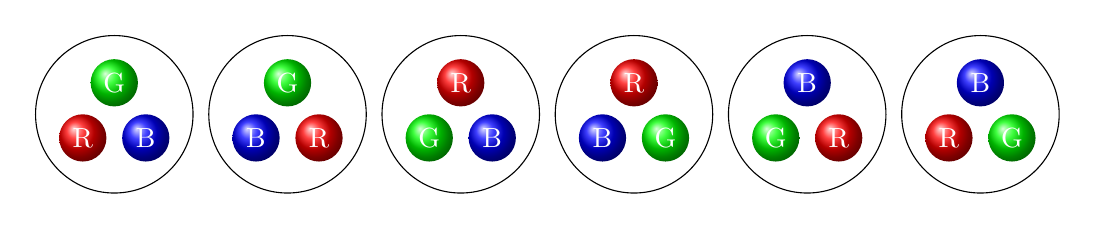
\begin{tikzpicture}[scale=1]
\clip (-1.1,-1.1) rectangle (12.1,1.1) ;  
\draw (0,0) circle (1cm) ; 
\shade[ball color=red]   (-0.4,-0.3)  node [white] {R} circle (0.3cm) ;
\shade[ball color=green] (   0, 0.4)  node [white] {G} circle (0.3cm) ;
\shade[ball color=blue]  ( 0.4,-0.3)  node [white] {B} circle (0.3cm) ;
\draw (2.2,0) circle (1cm) ;
\shade[ball color=blue]  (1.8,-0.3)   node [white] {B} circle (0.3cm) ;
\shade[ball color=green] (2.2, 0.4)   node [white] {G} circle (0.3cm) ;
\shade[ball color=red]   (2.6,-0.3)   node [white] {R} circle (0.3cm) ;
\draw (4.4,0) circle (1cm) ; 
\shade[ball color=green] (  4,-0.3)   node [white] {G} circle (0.3cm) ;
\shade[ball color=red]   (4.4, 0.4)   node [white] {R} circle (0.3cm) ;
\shade[ball color=blue]  (4.8,-0.3)   node [white] {B} circle (0.3cm) ;
\draw (6.6,0) circle (1cm) ; 
\shade[ball color=blue]  (6.2,-0.3)   node [white] {B} circle (0.3cm) ;
\shade[ball color=red]   (6.6, 0.4)   node [white] {R} circle (0.3cm) ;
\shade[ball color=green] (  7,-0.3)   node [white] {G} circle (0.3cm) ;
\draw (8.8,0) circle (1cm) ; 
\shade[ball color=green] (8.4,-0.3)   node [white] {G} circle (0.3cm) ;
\shade[ball color=blue]  (8.8, 0.4)   node [white] {B} circle (0.3cm) ;
\shade[ball color=red]   (9.2,-0.3)   node [white] {R} circle (0.3cm) ;
\draw (11,0) circle (1cm) ;
\shade[ball color=red]   (10.6,-0.3)  node [white] {R} circle (0.3cm) ;
\shade[ball color=blue]  (  11, 0.4)  node [white] {B} circle (0.3cm) ;
\shade[ball color=green] (11.4,-0.3)  node [white] {G} circle (0.3cm) ;                   
\end{tikzpicture}}{\Huge $\left.\vbox to 1.4cm {\vfil\hbox to 0cm{}\vfil}\right\rbrace$}

\vspace*{.3cm}

On a $\mathrm{card \;} \Omega = 6$. \\

Soit l'événement $E_1$ : « La boule verte est tombée dans le trou du haut. » \\
Soit l'événement $E_2$ : « La boule bleue est tombée dans le trou de droite. » \\

Les événements $E_1$ et $E_2$ ne sont pas incompatibles. \\
Les événements $E_1$ et $E_2$ sont-ils indépendants ? \\

\begin{itemize}
\item[•] On a $p\left(E_1 \cap E_2\right) = \dfrac{\mathrm{card \;}\left(E_1 \cap E_2\right)}{\mathrm{card \;} \Omega} = \dfrac{1}{6}$ \vspace*{.3cm} \\
\item[•] De plus, $p\left(E_1\right) \times p\left(E_2\right) = \dfrac{\mathrm{card \;} E_1}{\mathrm{card \;} \Omega} \times \dfrac{\mathrm{card \;} E_2}{\mathrm{card \;} \Omega} = \dfrac{2}{6} \times \dfrac{2}{6} = \dfrac{1}{9}$ \\
\end{itemize}

\vspace*{.3cm}

On a $p\left(E_1 \cap E_2\right) \neq p\left(E_1\right) \times p\left(E_2\right)$. \\

Donc $E_1$ et $E_2$ ne sont pas indépendants.

\newpage

\vspace*{-1cm}

\textbf{Exercice n°3 : Exercice type Bac} \\

On considère une usine d'horlogerie, dans laquelle la fabrication des montres se fait en deux phases. \\
La première phase fait apparaître le défaut « a » dans $2 \;$ \% des cas. \\
La seconde phase fait apparaître le défaut « b » dans $10 \;$ \% des cas. \\

Une montre est tirée au hasard. \\

On a l'événement $A$ : « La montre présente le défaut "a" ». \\
On a l'événement $B$ : « La montre présente le défaut "b" ». \\

On suppose que les événements $A$ et $B$ sont indépendants. \\

On considère les événements suivants :

\begin{itemize}
\item[•] $C$ : « La montre présente les deux défauts. »
\item[•] $D$ : « La montre ne présente aucun des deux défauts. »
\item[•] $E$ : « La montre présente un et un seul défaut . »
\end{itemize}

\vspace*{.3cm}

Déterminer $p\left(C\right)$, $p\left(D\right)$ et $p\left(E\right)$. \\

\textbf{Solution}

\begin{itemize}
\item[•] On a $C = A \cap B$, où $A$ et $B$ sont indépendants. \\

\begin{tabular}{lll}
\hspace*{-.3cm} D'où $p\left(C\right)$ & $=$ & $p\left(A \cap B\right)$ \\
& $=$ & $p\left(A\right) \times p\left(B\right)$ \\
& $=$ & $\dfrac{1}{50} \times \dfrac{1}{10}$ \vspace*{.2cm} \\
& $=$ & $\dfrac{1}{500}$ \\
\end{tabular}

\vspace*{.3cm}

\item[•] On a $D = \overline{C} \cap \overline{D}$. 

Or, d'après les lois de Morgan, $\overline{A} \cap \overline{B} = \overline{A \cup B}$. \\

\begin{tabular}{lll}
\hspace*{-.3cm} Donc $p\left(D\right)$ & $=$ & $p\left(\overline{A \cup B}\right)$ \\
& $=$ & $1 - p\left(A \cup B\right)$ \\
& $=$ & $1 - \left[p\left(A\right) + p\left(B\right) - p\left(A \cap B\right) \right]$ \\
& $=$ & $1 - \left(\dfrac{1}{50} + \dfrac{1}{10} - \dfrac{1}{500}\right)$ \\
& $=$ & $\dfrac{441}{500}$ \\
\end{tabular}

\vspace*{.3cm}

\item[•] On a $E = \left(A \cap \overline{B}\right) \cup \left(\overline{A} \cap B\right)$. \\
On a aussi $E = \overline{C} \cap \overline{D}$. 

Or, d'après les lois de Morgan, $\overline{C} \cap \overline{D} = \overline{C \cup D}$. \\

\begin{tabular}{lll}
\hspace*{-.3cm} Ainsi $p\left(E\right)$ & $=$ & $p\left(\overline{C \cup D}\right)$ \\
& $=$ & $1 - p\left(C \cup D\right)$ \\
& $=$ & $1 - \left[p\left(C\right) + p\left(D\right)\right]$ car $C$ et $D$ sont incompatibles. \\
& $=$ & $1 - \left(\dfrac{1}{500} + \dfrac{441}{500}\right)$ \\
& $=$ & $\dfrac{29}{250}$ \\
\end{tabular}

\vspace*{.3cm}

\textbf{Remarque :} On peut vérifier et on a bien $p\left(C\right) + p\left(D\right) + p\left(E\right) = 1$.

\vspace*{-50cm}
\end{itemize}

\vspace*{-50cm}

\newpage 

\vspace*{-2cm}

\subsection{Loi binomiale}

On considère une expérience n'admettant que deux résultats possibles, appelés « succès » ou « échec~» et notés \\ respectivement $S$ et $\overline{S} $. On effectue donc une \underline{épreuve de Bernoulli}. \\

On répète l'épreuve dans des conditions identiques, les résultats successifs étant indépendants les uns des autres. ON effectue donc un \underline{schéma de Bernoulli}.

\subsubsection{Exemple introductif}

On jette un dé non-pipé. \\ Soit un événement S : « On obtient un 6. » $p\left(S\right) = \dfrac{1}{6} $. \\

\underline{Épreuve de Bernoulli :} On jette le dé trois fois de suite. \\

\underline{Schéma de Bernoulli :} Soit \hbox{un événement S : « On obtient exactement deux fois 6 au cours des trois jets. »} \\

Quelle est la probabilité de S ? \\

\begin{tikzpicture} 
[level distance=10mm]
\tikzstyle{level 1}=[sibling distance=40mm]
\tikzstyle{level 2}=[sibling distance=20mm]
\tikzstyle{level 3}=[sibling distance=10mm]

\node (root) {}
[grow=right]
child {node {$\overline{S}$}
       child {node {$\overline{S}$}              
              child {node {$\overline{S}$}}
              child {node {$S$}} 
             }
       child {node {$S$}             
              child {node {$\overline{S}$}}
              child {node {$S$}} 
             }
      }
child {node {$S$}
       child {node {$\overline{S}$}
              child {node {$\overline{S}$}}
              child {node {$S$}} 
             }
       child {node {$S$}
              child {node {$\overline{S}$}}
              child {node {$S$}} 
             } 
      }
; 

\node at (root-2-2-2) [right] {$\qquad\qquad S\cap S\cap S \quad p(S)\times p(S) \times p(S) = \dfrac{1}{6} \times \dfrac{1}{6} \times \dfrac{1}{6} = \left(\dfrac{1}{6}\right)^3$} ; 
\node at (root-2-2-1) [right] {$\star \quad\qquad S\cap S\cap \overline{S} \quad p(S)\times p(S) \times p(\overline{S}) = \dfrac{1}{6} \times \dfrac{1}{6} \times \dfrac{5}{6} = \left(\dfrac{1}{6}\right)^2 \times \dfrac{5}{6}$} ; 
\node at (root-2-1-2) [right] {$\star \quad\qquad S\cap \overline{S}\cap S \quad p(S)\times p(\overline{S}) \times p(S) = \dfrac{1}{6} \times \dfrac{5}{6} \times \dfrac{1}{6} = \left(\dfrac{1}{6}\right)^2 \times \dfrac{5}{6}$} ; 
\node at (root-2-1-1) [right] {$\qquad\qquad S\cap \overline{S}\cap \overline{S} \quad p(S)\times p(\overline{S}) \times p(\overline{S}) = \dfrac{1}{6} \times \dfrac{5}{6} \times \dfrac{5}{6} = \dfrac{1}{6} \times \left(\dfrac{5}{6}\right)^2$} ; 
\node at (root-1-2-2) [right] {$\star \quad\qquad \overline{S}\cap S\cap S \quad p(\overline{S})\times p(S) \times p(S) = \dfrac{5}{6} \times \dfrac{1}{6} \times \dfrac{1}{6} = \left(\dfrac{1}{6}\right)^2 \times \dfrac{5}{6}$} ; 
\node at (root-1-2-1) [right] {$\qquad\qquad \overline{S}\cap S\cap \overline{S} \quad p(\overline{S})\times p(S) \times p(\overline{S}) = \dfrac{5}{6} \times \dfrac{1}{6} \times \dfrac{5}{6} = \dfrac{1}{6} \times \left(\dfrac{5}{6}\right)^2$} ; 
\node at (root-1-1-2) [right] {$\qquad\qquad \overline{S}\cap \overline{S}\cap S \quad p(\overline{S})\times p(\overline{S}) \times p(S) = \dfrac{5}{6} \times \dfrac{5}{6} \times \dfrac{1}{6} = \dfrac{1}{6} \times \left(\dfrac{5}{6}\right)^2$} ; 
\node at (root-1-1-1) [right] {$\qquad\qquad \overline{S}\cap \overline{S}\cap \overline{S} \quad p(\overline{S})\times p(\overline{S}) \times p(\overline{S}) = \dfrac{5}{6} \times \dfrac{5}{6} \times \dfrac{5}{6} = \left(\dfrac{5}{6}\right)^3$} ; 
\end{tikzpicture}

$ A = \left(S \cap S \cap \overline{S} \right) \cup \left(S \cap \overline{S} \cap S \right) \cup \left(\overline{S} \cap S \cap S\right)$. \\

Ces trois événements sont incompatibles deux à deux. \\

$ p\left(A\right) = p\left[\left(S \cap S \cap \overline{S} \right) \cup \left(S \cap \overline{S} \cap S \right) \cup \left(\overline{S} \cap S \cap S\right)\right] $ \\

$ p\left(A\right) = p\left(S \cap S \cap \overline{S} \right) + p\left(S \cap \overline{S} \cap S \right) + p\left(\overline{S} \cap S \cap S\right) $ \\

$ p\left(A\right) = \dfrac{1}{6} \times \dfrac{1}{6} \times \dfrac{5}{6} + \dfrac{1}{6} \times \dfrac{5}{6} \times \dfrac{1}{6} + \dfrac{5}{6} \times \dfrac{1}{6} \times \dfrac{1}{6} $ \\

$ p\left(A\right) =  \left(\dfrac{1}{6}\right)^2 \times \dfrac{5}{6} + \left(\dfrac{1}{6}\right)^2 \times \dfrac{5}{6} + \left(\dfrac{1}{6}\right)^2 \times \dfrac{5}{6} $ \\

$p\left(A\right) = 3 \left(\dfrac{1}{6} \right)^2 \times \dfrac{5}{6} $ \\

$ p\left(A\right) = \dfrac{5}{72} $

\vspace*{-5cm}

\newpage

\subsubsection{Généralisation}

Soit une épreuve de Bernoulli, avec $p$ la probabilité de succès de l'épreuve. \\
On répète l'épreuve $n$ fois dans des conditions identiques. \\ Les résultats étant indépendants les uns des autres. \\

\textbf{Schéma de Bernoulli de paramètres $\mathbf{n}$ et $\mathbf{p}$, ou loi binomiale :} $\mathbf{\mathcal{B} \left(n,p\right)}$ \\

Soit A l'événement « On obtient exactement k succès. » $p(A)$ est donnée par la formule : \\

$ p\left(A\right)  = \left(\begin{array}{c} n \\ k \end{array} \right) p^k \left(1-p\right)^{n-k} \; \;  $ avec $\left(\begin{array}{c} n \\ k \end{array} \right)$ le nombre de manières d'obtenir $k$ succès dans $n$ épreuves. \\

\textbf{Remarque :} On a $ 0 \leqslant k \leqslant n $.  \\

\textbf{Exemples :}

$\left(\begin{array}{c} 4 \\ 3 \end{array} \right)$ = 4. Il y a 4 façons d'obtenir trois succès quand l'épreuve est répétée quatre fois : \\

\begin{tabular}{l}
$ S \; S \; S \; \overline{S} $ \\
$ S \; S  \; \overline{S} \; S $ \\
$ S \; \overline{S} \; S \; S $ \\
$ \overline{S} \; S \; S \; S $ \\
\end{tabular}

\vspace{.3cm}

$\left(\begin{array}{c} 4 \\ 2 \end{array} \right)$ = 6. Il y a 6 façons d'obtenir deux succès quand l'épreuve est répétée quatre fois : \\

\begin{tabular}{l}
$ S \; S \; \overline{S} \; \overline{S} $ \\
$ S \; \overline{S} \; S \overline{S} $ \\
$ \overline{S} \; S \; S \overline{S} $ \\
$ S \; \overline{S}  \; \overline{S} \; S $ \\
$ \overline{S} \; S \; \overline{S} \; S $ \\
$ \overline{S} \; \overline{S} \; S \; S $ \\
\end{tabular}

\vspace{.3cm}

$\left(\begin{array}{c} 5 \\ 3 \end{array} \right)$ = 10. Il y a 10 façons d'obtenir trois succès quand l'épreuve est répétée cinq fois : \\

\begin{tabular}{l}
$ S \; S \; S\; \overline{S} \; \overline{S} $ \\
$ S \; S \overline{S} \; S \; \overline{S} $ \\
$ S \; \overline{S} \; S \; S \; \overline{S} $ \\
$ \overline{S}  \; S \; S \; S \overline{S} $ \\
$ S \; S \;  \overline{S} \; \overline{S} \; S $ \\
$ S \; \overline{S} \; S \; \overline{S} \; S $ \\
$ \overline{S} \; S \; S \; \overline{S} \; S $ \\
$ S \; \overline{S} \; \overline{S} \; S \; S $ \\
$  \overline{S} \; S \; \overline{S} \; S \; S $ \\
$  \overline{S} \; \overline{S} \; S \; S \; S $ \\
\end{tabular}

\vspace{.3cm}

\subsubsection{Triangle de Pascal}

\begin{tabular}{r@{$\;=\;$}lll}
\multicolumn{2}{l}{$\;\;\; a+b$} & $1 \;\;\; 1$ & $n=1$ \\
$(a+b)^2 $ & $ a^2 +2ab+b^2$ & $1 \;\;\; 2 \;\;\; 1 $ & $n =2$ \\
$(a+b)^3 $ & $ a^3 +3a^2b+3ab^2+b^3$ & $1 \;\;\; 3 \;\;\; 3 \;\;\;\; 1 $ & $n =3$ \\
$(a+b)^4 $ & $ a^4 + 4a^3b +6a^2 b^2 + 4ab^3 +b^4 $
           &  $1 \;\;\; 4 \;\;\; 6 \;\;\;\; 4 \;\;\;\; 1 $ & $n =4$ \\
$(a+b)^5 $ & $ a^5 + 5a^4b +10a^3 b^2 + 10a^2b^3 + 5ab^4 + b^5 $
           &  $1 \;\;\; 5 \; 10 \; 10 \;\;\;  5 \;\; 1 $ & $n =5$ \\    
$(a+b)^6 $ & $ a^6 + 6a^5b +15a^4 b^2 + 20a^3b^3 + 15a^2b^4 + 6ab^5 +b^6 $
           &  $1 \;\;\; 6 \; 15 \; 20 \; 15 \;  6 \;\;\; 1 $ & $n =6$ \\                     
\end{tabular}\\

\textcolor{orange} {\begin{tabular}{lccc}
Calculatrice : & 3 & combinaison & 2 \\
& 4 & combinaison & 2 \\
& 4 & combinaison & 3 \\
& 5 & combinaison & 3 \\
\end{tabular}}

\vspace*{.3cm}

\makeatletter
\newcommand\binomialCoefficient[2]{%
    % Store values 
    \c@pgf@counta=#1% n
    \c@pgf@countb=#2% k
    %
    % Take advantage of symmetry if k > n - k
    \c@pgf@countc=\c@pgf@counta%
    \advance\c@pgf@countc by-\c@pgf@countb%
    \ifnum\c@pgf@countb>\c@pgf@countc%
        \c@pgf@countb=\c@pgf@countc%
    \fi%
    %
    % Recursively compute the coefficients
    \c@pgf@countc=1% will hold the result
    \c@pgf@countd=0% counter
    \pgfmathloop% c -> c*(n-i)/(i+1) for i=0,...,k-1
        \ifnum\c@pgf@countd<\c@pgf@countb%
        \multiply\c@pgf@countc by\c@pgf@counta%
        \advance\c@pgf@counta by-1%
        \advance\c@pgf@countd by1%
        \divide\c@pgf@countc by\c@pgf@countd%
    \repeatpgfmathloop%
    \the\c@pgf@countc%
}
\makeatother

\begin{tikzpicture}
\foreach \n in {0,...,9} {
  \foreach \k in {0,...,\n} {
    \node at (\k-\n/2,-\n) {$\binomialCoefficient{\n}{\k}$};
  }
}
\end{tikzpicture}

\newpage

\subsubsection{Amusette}

Il naît 1044 garçons pour 1000 filles. \\ Quelle est la probabilité qu'il y ait 3 garçons pour 5 familles de 5 enfants ? \\

Épreuve de Bernoulli : Faire un enfant. \\

Succès $S$ : « Avoir un garçon. » $p\left(S\right) = \dfrac{1044}{2044} = \dfrac{261}{511} $ \\

On répète l'épreuve 5 fois. \\

Schéma de Bernoulli de paramètre $n = 5 $ et $p = \dfrac{1044}{2044} $ \\

Soit un événement A : « On obtient exactement trois garçons. » \\

$p\left(X = 3\right) = \left(\begin{array}{c} 3 \\ 5 \end{array}\right) \left(\dfrac{261}{511}\right)^3\left(\dfrac{1000}{2044}\right)^2$ \\

$p\left(X=3\right) = 10 \times \left(\dfrac{261}{511}\right)^3\left(\dfrac{1000}{2044}\right)^2 $ \\

$ p\left(X=3\right)  \approx 0,3189 $ \\

\textcolor{orange}{À la calculatrice : $\mathrm{binompdf} \left(5,\dfrac{261}{511},3\right)$} 

\newpage

\vspace*{-1cm}

\subsubsection{Exercice}

On effectue une enquête auprès des employés d'une entreprise. 

Pendant une période donnée, la durée de congés de $20 \;$ \% d'entre-eux est supérieure à $25$ jours. 

On interroge un employé au hasard. 

On désigne par $A$ l'événement : « Le congé de l'employé interrogé est supérieur à $25$ jours ». 

On interroge $4$ personnes au hasard. 

On désigne par $X$ le nombre de personnes pour lesquelles l'événement $A$ est réalisé. 

On cherche la loi de probabilité de $X$. \\

Compléter le tableau suivant : \\

\begin{tabular}{|c|c|c|c|}
\hline
& Formule & Forme Fractionnaire & Forme décimale \\
\hline
& & & \\
$p\left(X = 0\right)$ & & & \\ 
& & & \\
\hline
& & & \\
$p\left(X = 1\right)$ & & & \\ 
& & & \\
\hline
& & & \\
$p\left(X = 2\right)$ & & & \\ 
& & & \\
\hline
& & & \\
$p\left(X = 3\right)$ & & & \\ 
& & & \\
\hline
& & & \\
$p\left(X = 4\right)$ & & & \\ 
& & & \\
\hline
\end{tabular}

\vspace*{.3cm}

\textbf{Solution} \\

\begin{tabular}{|c|c|c|c|}
\hline
& Formule & Forme Fractionnaire & Forme décimale \\
\hline
& & & \\
$p\left(X = 0\right)$ & \color{red} $1 \times \left(\dfrac{4}{5}\right)^4$ \color{black} & \color{red} $\dfrac{256}{625}$ \color{black} & \color{red} $0,4096$ \color{black} \\ 
& & & \\
\hline
& & & \\
$p\left(X = 1\right)$ & \color{red} $4 \times \dfrac{1}{5} \times \left(\dfrac{4}{5}\right)^3$ \color{black} & \color{red} $\dfrac{256}{625}$ \color{black} & \color{red} $0,4096$ \color{black} \\ 
& & & \\
\hline
& & & \\
$p\left(X = 2\right)$ & \color{red} $6 \times \left(\dfrac{1}{5}\right)^2 \times \left(\dfrac{4}{5}\right)^2$ \color{black} & \color{red} $\dfrac{96}{625}$ \color{black} & \color{red} $0,1536$ \color{black} \\ 
& & & \\
\hline
& & & \\
$p\left(X = 3\right)$ & \color{red} $4 \times \left(\dfrac{1}{5}\right)^3 \times \dfrac{4}{5}$ \color{black} & \color{red} $\dfrac{16}{625}$ \color{black} & \color{red} $0,0254$ \color{black} \\ 
& & & \\
\hline
& & & \\
$p\left(X = 4\right)$ & \color{red} $1 \times \left(\dfrac{1}{5}\right)^4$ \color{black} & \color{red} $\dfrac{1}{625}$ \color{black} & \color{red} $0,0016$ \color{black} \\ 
& & & \\
\hline
\end{tabular}

\vspace*{-5cm}

\newpage

\subsection{Variable aléatoire et espérance mathématique}

\subsubsection{Exemple}

On investit un euro. \\ On tire une carte dans un jeu de 52 cartes. On gagne 4 euros si la carte tirée est un cœur. On perd sa mise sinon. \\

\begin{itemize}
\item[•] Soit $X$ la \textbf{variable aléatoire} qui correspond au gain du jouer. \\ 

$X\left(\Omega\right) = \lb -1 \; ; \; 3 \rb$. \\
\item[•] \textbf{Loi de probabilité} de $X$ : \\
\end{itemize}

\begin{tabular}{|c|l|l|}
\hline
$x_i$ & $-1$ & $3$ \\
\hline
& & \\
$p\left(X = x_i\right)$ & $\dfrac{3}{4}$ & $\dfrac{1}{4}$ \\
& & \\
\hline
\end{tabular}

\vspace*{.3cm}

On a bien $p\left(X = -1\right) + p\left(X = 3\right) = 1$ \\

\begin{itemize}
\item[•] \textbf{Espérance mathématique} de X : \\
\end{itemize}

$E(x) = \displaystyle \sum  x_ip\left(X = x_i\right)$ \\

$ E(x) = -1 \times \dfrac{3}{4} + 3 \times \dfrac{1}{4} = 0$. \\

Donc le jeu est équilibré. \\

L'espérance mathématique s'apparente à la moyenne des gains, car on peut écrire : \\

$E(x) = \dfrac{3 \times \left(-1\right)+ 1 \times 3}{4}$, qui est de la forme : $\overline{x} = \dfrac{\Sigma n_ix_i}{\Sigma n_i}$ \\

\textbf{Remarque :} \\

\begin{itemize}
\item[*] Si $E(x) > 0$, alors le jeu est favorable au joueur.  
\item[*] Si $E(x) < 0$, alors le jeu est défavorable au joueur. 
\end{itemize} 

\newpage

\subsubsection{Sujet de bac}

Un fabricant d'objets périssables : \\

\begin{itemize}
\item[•] gagne $300$ euros par objet vendu.
\item[•] perd $200$ euros par objet invendu. 
\end{itemize}

\vspace*{.3cm}

On appelle $D$ la demande journalière. \\
On appelle $G_k$ la variable aléatoire correspondant au gain quotidien réalisé lorsque l'on fabrique $k$ objets avec $0 \leqslant k \leqslant 4$. \\

On donne : \\

\begin{tabular}{|c|c|c|c|c|c|c|}
\hline
& & & & & & \\
Demandes journalières $d_i$ & 0 & 1 & 2 & 3 & 4 & 5 ou plus \\
& & & & & & \\
\hline
& & & & & & \\
$p\left(D = d_i\right)$ & $0,1$ & $0,2$ & $0,35$ & $0,25$ & $0,1$ & $0$ \\
& & & & & & \\
\hline
& & & & & & \\
$G_1$ & $-200$ & $300$ & $300$ & $300$ & $300$ & $300$ \\
& & & & & & \\
\hline
& & & & & & \\
$G_2$ & $-400$ & $100$ & $600$ & $600$ & $600$ & $600$ \\
& & & & & & \\
\hline
& & & & & & \\
$G_3$ & $-600$ & $-100$ & $400$ & $900$ & $900$ & $900$ \\
& & & & & & \\
\hline
& & & & & & \\
$G_4$ & $-800$ & $-300$ & $200$ & $700$ & $1200$ & $1200$ \\
& & & & & & \\
\hline
\end{tabular}

\vspace*{.3cm}

On calcule l'espérance mathématique des différents gains : \\

$E(G_1) = -200 \times 0,1 + 300 \times 0,2 + 300 \times 0,35 + 300 \times 0,25 + 300 \times 0,1$ \\
$E(G_1) = 250$ \\

De même, on trouve : \\ 

$E(G_2) = 400$ \\

$E(G_3) = 375$ \\

$E(G_4) = 225$ \\

Donc l'artisan doit fabriquer $2$ objets pour espérer obtenir la gain le plus important. \\ La moyenne de ses gains sera alors de $400$ euros par jour.

\newpage

\vspace*{-1.5cm}

\subsection{Écart-type}

\vspace*{.2cm}

\textbf{Exemple :} Le jeu de la roulette. \\

Sur une roulette, on a $37$ numéros : $0$, $1$, $2$, $3$, ... Deux possibilités de jeu existent : \\

\begin{itemize}
\item[1.] Chance pleine \\

On joue un numéro. \\

\begin{itemize}
\item[•] Si on gagne, on gagne $36$ fois la mise. 
\item[•] Si on perd, on perd sa mise. 
\end{itemize}

\vspace*{.3cm}

\item[2.] Chances simples \\

On a $18$ numéros rouges. De même, on a $18$ numéros noirs. \\
$18$ numéros « manqué » de $1$ à $18$. $18$ numéros « passé » de $19$ à $36$. \\

\begin{itemize}
\item[•] Si on gagne, on gagne deux fois sa mise. 
\item[•] Si on perd, on perd sa mise. 
\end{itemize}

\end{itemize}

\vspace*{.3cm}

On joue $1$ euro. \\
On note $X$ la variable aléatoire correspondant aux gains réels du joueurs. \\

On étudie les deux cas possibles. On cherche les lois de probabilités dans les deux possibles, ainsi que l'espérance dans chacun des cas. \\

\begin{itemize}
\item[1.] \textbf{Chance pleine} : On a $X\left(\Omega\right) = \lbb -1 \; ; \; 35 \rbb$. \\

On a alors le tableau suivant : \\

\begin{tabular}{c|c|c}
$x_i$ & $-1$ & $35$ \\
\hline
& \\
$p\left(X = x_i\right)$ & $\dfrac{36}{37}$ & $\dfrac{1}{37}$ \\
& \\
\end{tabular}

\vspace*{.3cm}

On a $E\left(X\right) = -1 \times \dfrac{36}{37} + \dfrac{35}{37} = -\dfrac{1}{37} \approx -0,027$. \\

\item[2.] \textbf{Chances simples} : On a $X\left(\Omega\right) = \lbb -1 \; ; \; 1 \rbb$. \\

On a alors le tableau suivant : \\

\begin{tabular}{c|c|c}
$x_i$ & $-1$ & $1$ \\
\hline
& \\
$p\left(X = x_i\right)$ & $\dfrac{19}{37}$ & $\dfrac{158}{37}$ \\
& \\
\end{tabular}

\vspace*{.3cm}

On a $E\left(X\right) = -1 \times \dfrac{19}{37} + 1 \times \dfrac{18}{37} = -\dfrac{1}{37} \approx -0,027$. 
\end{itemize}

\vspace*{-10cm}

\newpage

Les espérances sont les mêmes, alors que les jeux sont différents. On définit donc l'écart-type de la variable aléatoire $X$ par $\sigma\left(X\right) = \sqrt{E\left(X^2\right) - \left[E\left(X\right)\right]^2}$. \\

On calcule l'écart-type de la variable aléatoire $X$ dans les deux : \\

\begin{itemize}
\item[1.] Chance pleine : \\

On a $E\left(X\right) = -\dfrac{1}{37}$. \vspace*{.3cm} \\

De plus, $E\left(X^2\right) = \left(-1\right)^2 \times \dfrac{36}{37} + 35^2 \times \dfrac{1}{37} = \dfrac{1261}{37}$. \vspace*{.3cm} \\

On a $\sigma\left(X\right) = \sigma\left(X\right) = \sqrt{E\left(X^2\right) - \left[E\left(X\right)\right]^2}$. \vspace*{.3cm} \\

D'où $\sigma\left(X\right) = \sqrt{\dfrac{1261}{37} - \left(-\dfrac{1}{37}\right)^2} \approx 5,838$. \\

\item[2.] Chances simples : \\

On a $E\left(X\right) = -\dfrac{1}{37}$. \vspace*{.3cm} \\

De plus, $E\left(X^2\right) = \left(-1\right)^2 \times \dfrac{19}{37} + 1^2 \times \dfrac{18}{37} = 1$. \vspace*{.3cm} \\

On a $\sigma\left(X\right) = \sigma\left(X\right) = \sqrt{E\left(X^2\right) - \left[E\left(X\right)\right]^2}$. \vspace*{.3cm} \\

D'où $\sigma\left(X\right) = \sqrt{1 - \left(-\dfrac{1}{37}\right)^2} \approx 0,9996$. \\
\end{itemize}

\vspace*{.3cm}

Ainsi, si le joueur est enthousiaste, il choisira de jouer au jeu de la chance pleine. Cependant, si le joueur est prudent, il choisira de jouer au jeu des chances simples. 


\ifdefined\COMPLETE
\else
    \end{document}
\fi